\documentclass[12pt,a4paper]{article}

\usepackage{graphicx}                            % Para poder incluir gráficos.
\usepackage[brazilian]{babel}                    % Para separar as sílabas, e colocar os nomes padrão (capítulo, bibliografia, etc.) em português.
\usepackage[utf8]{inputenc}                      % Para poder escrever diretamente com acentos, sem ter que usar códigos.
\usepackage[T1]{fontenc}                         % Para poder copiar do PDF acentos.
\usepackage{natbib}                              % \citep{jon90} --> (Jones et al., 1990)
\usepackage[colorlinks,citecolor=blue]{hyperref} % Para colocar links nas referências, equações, figuras, etc, além de menu árvore no PDF.
\usepackage{verbatim}                            % Para poder comentar regiões do arquivo .tex 
\usepackage[small,bf]{caption}                   % Para que legendas de figuras e tabelas fique em fonte menor e com negrito.
\usepackage{amssymb}                             % Para poder utilizar alguns símbolos matemáticos especiais.
\usepackage{amsmath}                             % Para poder usar o comando 'cases', e possivelmente outros.
\usepackage{fancyhdr}                            % Para poder fazer cabeçalhos e rodapés mais bonitos.
%\usepackage{epstopdf}                            % Para poder usar imagens .eps no compilador pdflatex (que permite usar imagens .png).
\usepackage{times}                               % Para usar typeset bem definido.
\usepackage{titlesec}                            % Para poder redefinir o formato dos títulos de seções
\usepackage[svgnames]{xcolor}                    % Várias cores (+150)                         
\usepackage{helvet}                              % Fonte helvética
\usepackage{lipsum}                              % Para preencher com texto. 


%%% Formatting %%%
% Cores:
\definecolor{MSBlue}{rgb}{.204,.353,.541}
\definecolor{MSLightBlue}{rgb}{.31,.506,.741}
\newcommand{\secColor}{\color{RoyalBlue}}
% Título das seções:
\titleformat*{\section}{\LARGE\bfseries\sffamily\secColor}
\titleformat*{\subsection}{\Large\bfseries\sffamily\secColor}
\titleformat*{\subsubsection}{\normalsize\bfseries\sffamily\secColor}
\renewcommand{\headrule}{\secColor\hrule}
% Header:
\pagestyle{fancy}
\setlength\headheight{26pt} %% just to make warning go away. Adjust the value after looking into the warning.
\fancyhead[L]{\fontsize{10}{12}\sffamily\secColor\rightmark}
\rhead{
\includegraphics[width=3cm]{acredito_fundobranco.png}}
% My commands %
\newcommand{\myurl}[1]{{\tiny\url{#1}}}


\author{Henrique S. Xavier \& João Carabetta}
\title{\Huge\sffamily\bfseries 100 dias de congresso}



%%%%%%%%%%%%%%%% REPORT %%%%%%%%%%%%%%%%%%
\begin{document}

% Página de rosto:
\pagenumbering{gobble}
\thispagestyle{empty}
\maketitle
%\tableofcontents
\pagebreak

% Relatório mesmo:
\thispagestyle{plain}
\pagenumbering{arabic}

%%%%%%%%%%%%%%%%%%%
\section{Introdução}
\label{sec:intro}

Este trabalho visa apresentar um panorama do congresso nacional brasileiro nos 100 primeiros dias da $56^{\mathrm{\underline{a}}}$ legislatura, que
se iniciou no dia 1 de fevereiro de 2019, utilizando as bases de dados abertos da câmara\footnote{\myurl{http://dadosabertos.camara.leg.br/}}
e do senado\footnote{\myurl{http://www12.senado.leg.br/dados-abertos}}. Além de apresentar o cenário atual, também buscamos analisar
as características históricas do congresso, tanto para fins de comparação quanto de construção de um retrato de suas características
mais estruturais. Os objetivos deste relatório são dois: de servir de subsídio para a atividade parlamentar do movimento Acredito na
câmara e no senado, e de prover à sociedade mais informações relativas ao trabalho de seus representantes e das estruturas governamentais
utilizadas nessa representação.

Dado o curto período de tempo disponível para a realização deste estudo, apresentamos aqui uma análise inicial que
certamente poderá ser desdobrada e aprofundada em investigações futuras. Essa análise foi segmentada em duas frentes,
uma focada nos parlamentares e outra nas proposições -- e.g. projetos de lei (PLs), medidas provisórias (MPs) e propostas
de emendas à constituição (PECs) -- em tramitação.

Em relação aos parlamentares, buscamos investigar:
(\emph{i}) o uso da cota parlamentar (verba destinada a cobrir os custos do trabalho parlamentar);
(\emph{ii}) o apoio ao governo e a fidelidade partidária;
(\emph{iii}) a distribuição de cargos e poder;
(\emph{iv}) e o nível de participação e engajamento.
Em relação às proposições, analisamos quais temas são os mais recorrentes historicamente e na atual legislatura.

Um de nossos primeiros achados se refere à limitação das bases de dados, particularmente em relação
aos dados mais recentes. Por exemplo, os parlamentares tem um prazo de 90 dias para solicitar reembolso
à cota parlamentar\footnote{\myurl{https://www2.camara.leg.br/comunicacao/assessoria-de-imprensa/cota-parlamentar}}
e empresas aéreas chegam a demorar mais do que isso para comunicar à câmara a emissão de
bilhetes, o que torna incompleta a amostra de gastos dos últimos 100 dias. Nesses casos, optamos por apenas
realizar uma análise histórica.


%%%%%%%%%%%%%%%%%%%%%%
\section{Parlamentares}


%%%%%%%%%%%%%%%%%%%%%%%%%%%%%%%%%%%
\subsection{Uso da cota parlamentar}

Conforme apresentado na Seção \ref{sec:intro}, as bases de dados relacionadas às despesas parlamentares dos 100 últimos
dias ainda estão sendo atualizadas. As referentes ao ano de 2018 ganharam, em média, 530 entradas por dia desde o início
dessa análise, em grande parte relativas à emissão de bilhetes aéreos. Essa incompleteza da base de dados se evidencia
na Fig. \ref{fig:n-despesas-por-mes}. A queda abrupta, a partir de 2018, no número de despesas registradas é ao menos
em parte consequência dessa defasagem no registro dos gastos. A Fig. \ref{fig:n-despesas-por-mes} ainda mostra que
os gastos do total de deputados segue um padrão recorrente ao longo dos anos, com uma queda significativa em janeiro.

\begin{figure}[t]
\centering
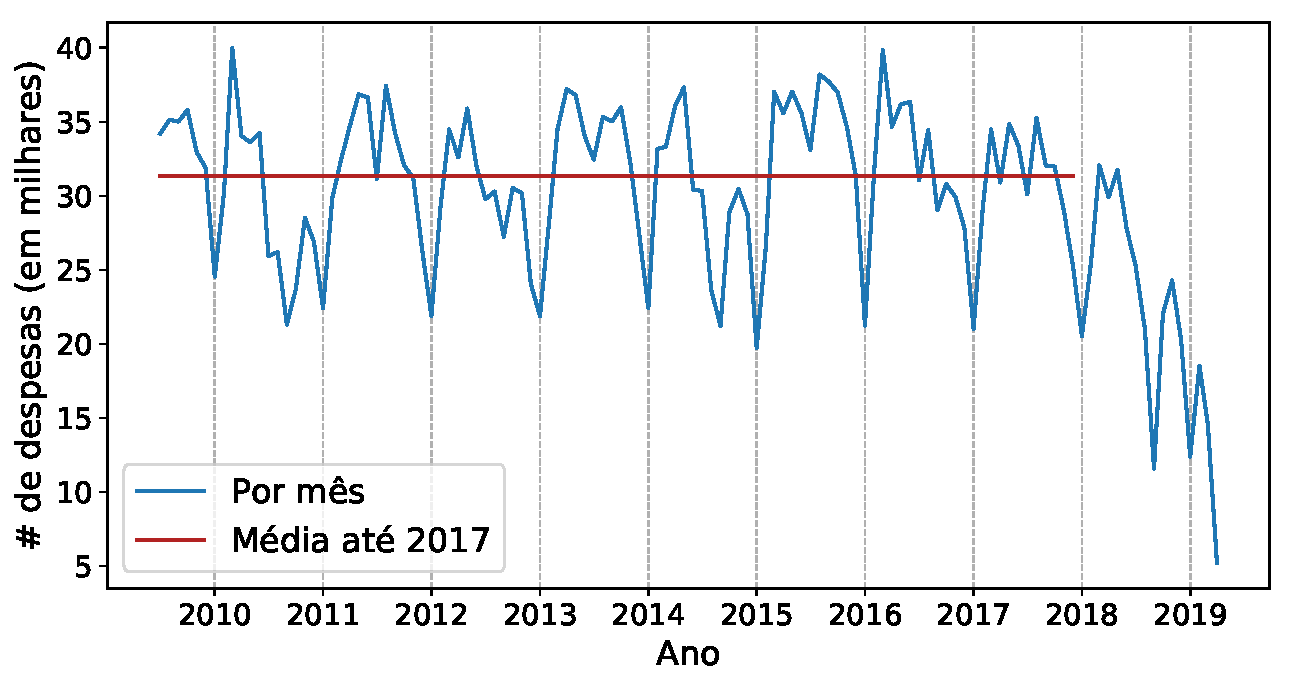
\includegraphics[width=1.0\textwidth]{graficos/n_despesas_por_mes_2019-04-29.pdf}
\caption{Número de despesas na base de dados de uso da cota parlamentar dos deputados federais
  referentes a cada mês, em função do tempo (em azul).
  A linha vermelha indica o número médio de 2009 a 2018.}
\label{fig:n-despesas-por-mes}
\end{figure} 

Para acompanhar o valor total gasto com a cota parlamentar ao longo do tempo, nós primeiro deflacionamos os
valores pelo IPCA e em seguida o decompusemos num modelo aditivo com termos de tendência geral, sazonalidade e
resíduo (veja a Fig. \ref{fig:total-despesas-por-mes}). Através da curva de tendência, podemos notar que
o valor médio gasto praticamente não se alterou desde 2010, sendo que uma leve queda pode ser notada em anos
recentes. Ressaltamos que ao menos parte dessa queda é consequência da defasagem de registro dos gastos.

\begin{figure}[t]
\centering
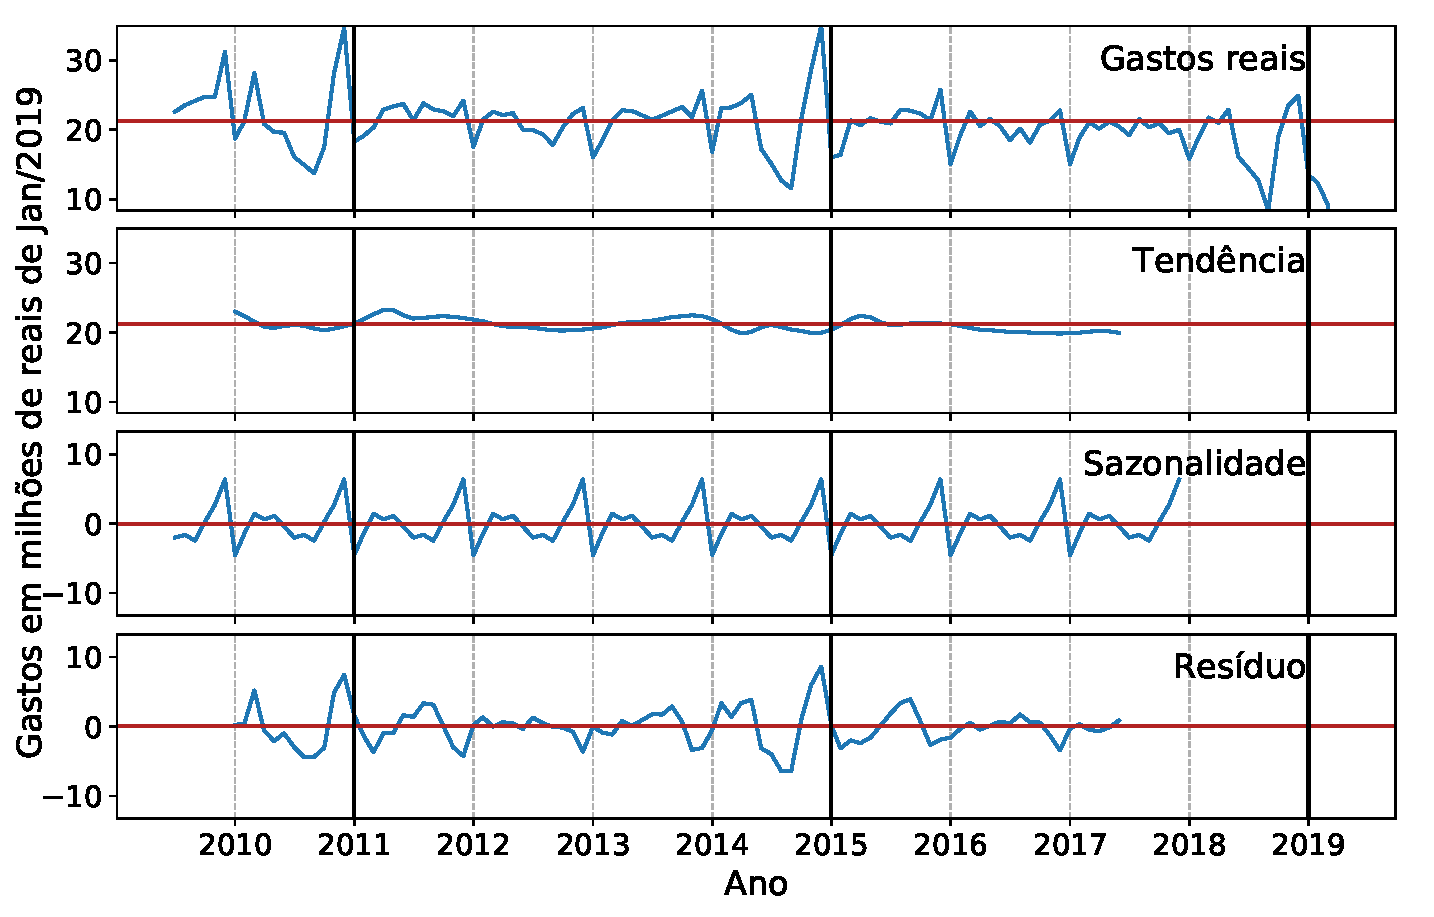
\includegraphics[width=1.0\textwidth]{graficos/despesas-reais-e-sazonalidade_2019-04-29.pdf}
\caption{Valor real (descontada a inflação) gasto com o exercício da atividade parlamentar em cada mês
  (reembolsos feitos dentro da cota parlamentar, em azul). O painel superior mostra o valor observado, e os
  abaixo mostram as contribuições de: tendência geral, calculada através de uma média móvel; sazonalidade; e resíduo.
  A linha vermelha indica o valor médio em todo o período (nos dois painéis superiores) e o zero (nos dois
  painéis inferiores). A decomposição em contribuições aditivas foi feita até o ano de 2017.}
\label{fig:total-despesas-por-mes}
\end{figure} 

Também é possível notar que os gastos apresentam uma sazonalidade bastante marcada, com quedas mais
acentuadas em janeiro e picos em dezembro. Esses picos podem decorrer do fato de que a cota parlamentar, mensal,
pode ser acumulada ao longo do ano mas não pode ser transferida para o exercício financeiro seguinte.
É possível percebem ainda, tanto nos gráficos do valor observado quanto no de resíduos, que existe
um pico ainda mais acentuado ao final de cada legislatura (marcadas com linhas verticais pretas contínuas).
Esse pico parece ser precedido por uma queda nos gastos, possivelmente indicando uma estratégia de acúmulo de verba
para a realização de um último gasto em dezembro.

Por fim, verificamos como o valor total reembolsado pela cota parlamentar se divide nas categorias pré-definidas
pela câmara. A Figura \ref{fig:despesas-por-tipo} mostra a fração do valor total que é destinada a cada categoria
de gastos. Verificamos que os maiores gastos realizados são com divulgação da atividade parlamentar (que, em geral,
apresentam valores altos para uma única despesa e perfazem 20\% do total) e com transporte aéreo: somando as rubricas
``emissão de bilhere aéreo'', ``locação ou fretamento de aeronaves'' e ``passagens aéreas'', temos cerca de
23\% dos gastos. Em grande medida, esse montante deriva do deslocamento semanal do deputado ao seu estado de origem.
Gastos com manutenção de escritório de apoio em seu estado, consultorias, telefonia e transportes terrestres vêm
em seguida. Junto com passagens aéreas, o transporte totaliza cerca de 44\% do total. Gastos com alimentação e
hospedagem fora do distrito federal totalizam, em média, menos de 2\% dos gastos.

\begin{figure}[t]
\centering
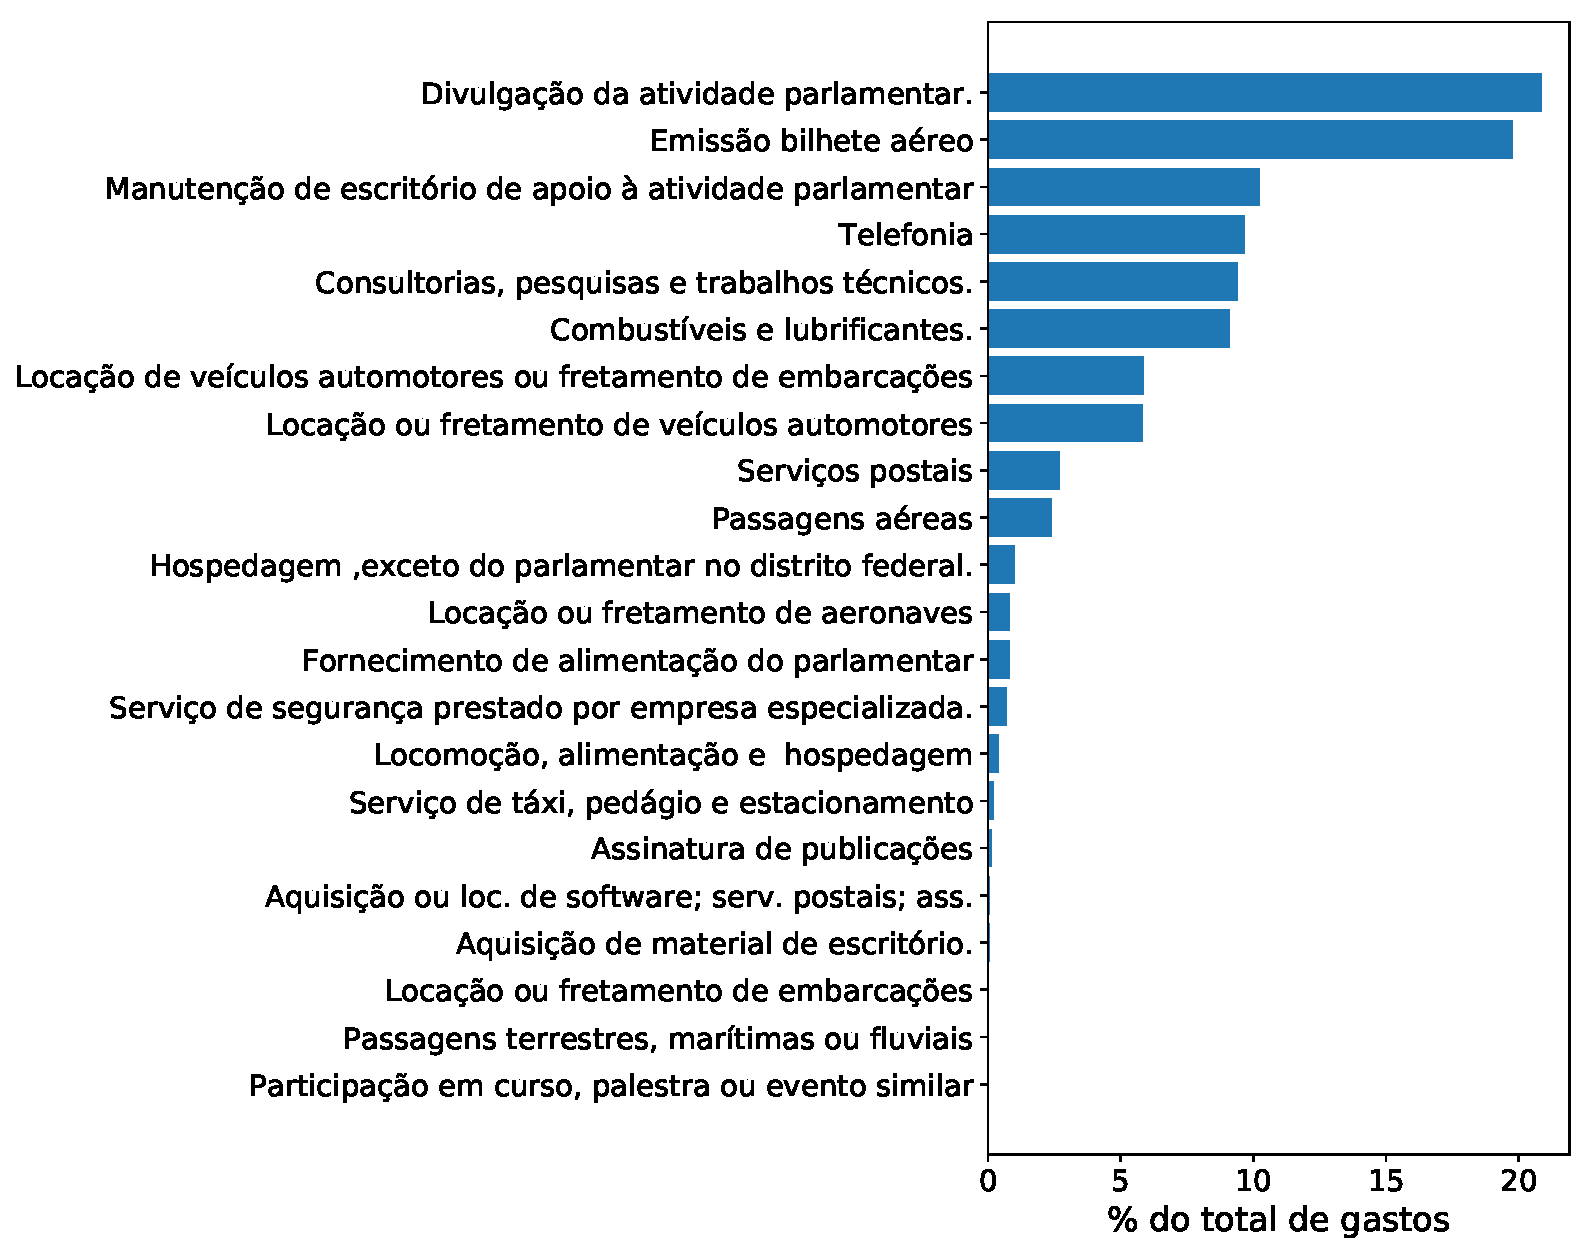
\includegraphics[width=1.0\textwidth]{graficos/total-despesas-por-tipo_2019-04-29.pdf}
\caption{Porcentagem do valor total utilizado pelos deputados federais que é destinado a cada finalidade. Nesse
cálculo, utilizamos os valores de 2009 a 2017, corrigigos pela inflação.}
\label{fig:despesas-por-tipo}
\end{figure} 


%%%%%%%%%%%%%%%%%%%%%%%%%%%%%%%%
\subsection{Análise das votações}

\subsubsection{Apoio ao governo}

Podemos estimar o apoio ao governo através da correlação entre os votos dos parlamentares e a orientação de voto
dada pelo governo. Para fins de comparação, realizamos esse estudo para os 100 primeiros dias da presente legislatura
e das legislaturas anteriores, desde 1999. Votações nas quais não existia orientação do governo foram ignoradas.

A Fig. \ref{fig:apoio-governo-deputados} mostra a distribuição de deputados e deputadas em função do grau de
alinhamento com a orientação do governo, nos 100 primeiros dias de legislatura, desde 1999 até hoje.
Na maioria dos casos, é possível notar um grupo significativo de deputados que vota 90\% das vezes ou mais em acordo com o governo.
No caso de 1999 (início do segundo mandato de Fernando Henrique Cardoso), mais da metade dos deputados votaram
com o governo 100\% das vezes, levando a mediana a esse valor. No início do segundo mandato de Dilma Rousseff,
esse grupo se dilui e o alinhamento dos deputados se torna bastante disperso.

\begin{figure}[t]
\centering
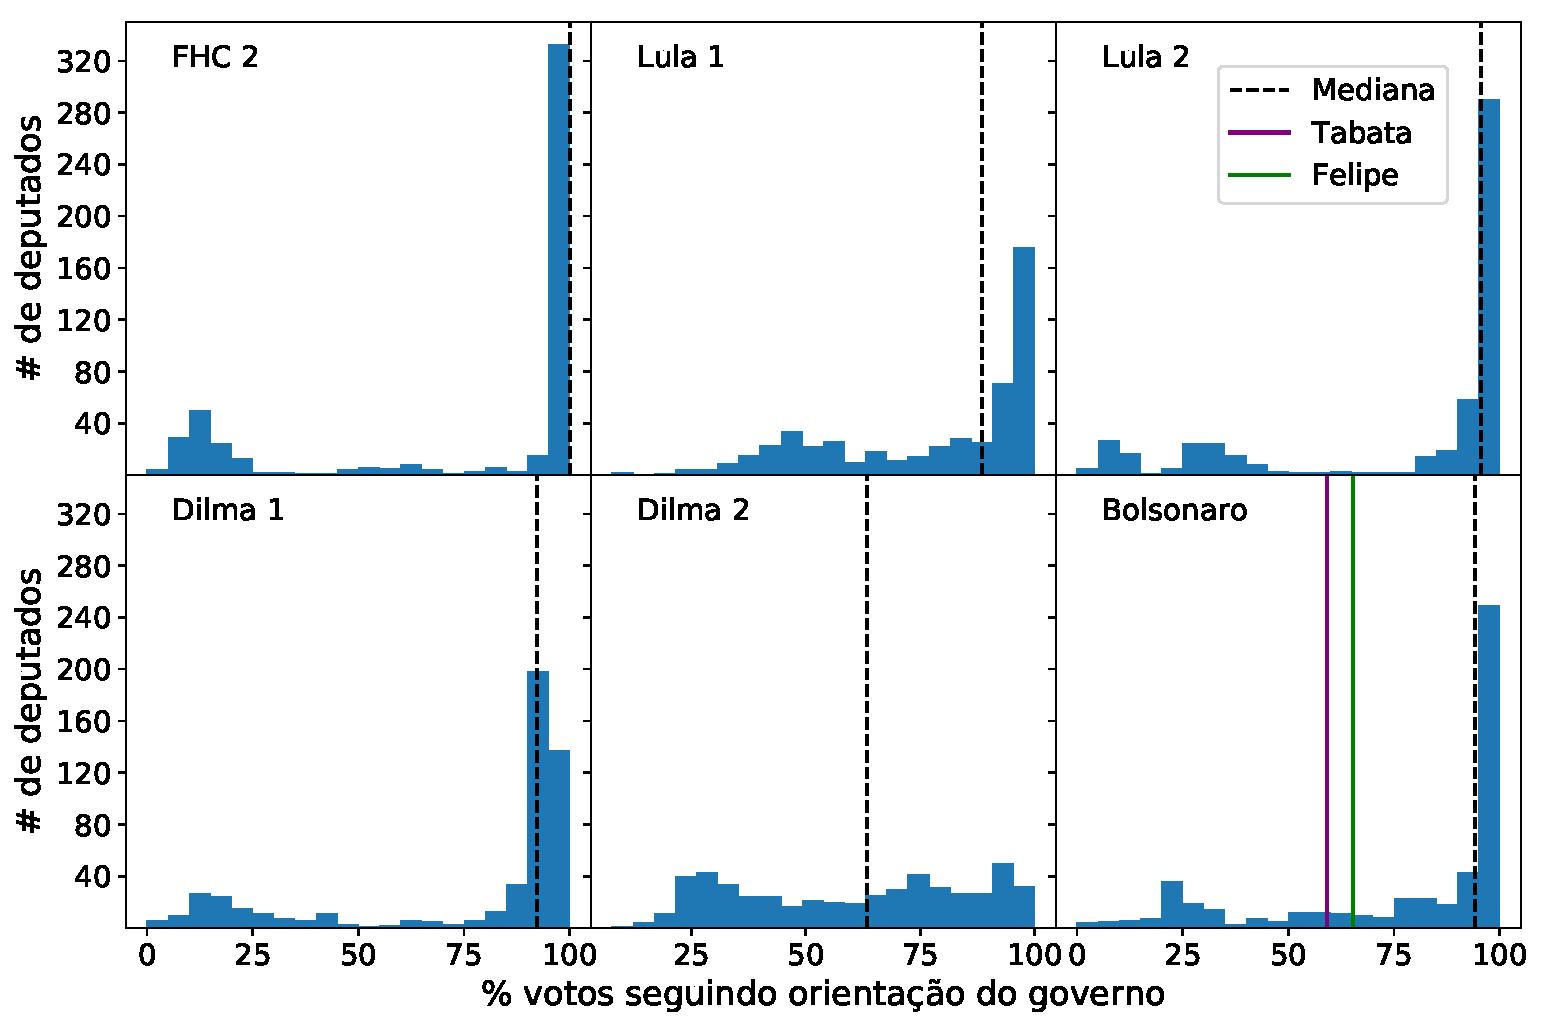
\includegraphics[width=1.0\textwidth]{graficos/apoio_ao_governo_deputados_2019-04-30.pdf}
\caption{Contagem do número de deputados em função da fração de seus votos no plenário que se
  alinham com a orientação do governo. Cada painel apresenta os dados dos 100 primeiros dias de
  cada legislatura, discriminadas pelo presidente no período. A linha vertical tracejada preta
  separa a metade dos deputados com maior e menor apoio e as linhas coloridas indicam a posição
  dos parlamentares do Acredito.}
\label{fig:apoio-governo-deputados}
\end{figure} 

Na maioria das legislaturas, a distribuição bimodal indica uma separação clara dos deputados
entre governo e oposição, sendo esta última contrária ao governo em mais de 2/3 das vezes.
Esse padrão se altera no primeiro mandato de Luiz Inácio Lula da Silva e no segundo mandato de Dilma.

A Fig. \ref{fig:apoio-governo-deputados} ainda indica que o governo de Jair Messias Bolsonaro detém
razoável apoio dos deputados, com distribuição similar à de governos anteriores. Esse dado contrasta
com a impressão derivada da cobertura da mídia, conforme mostra as manchetes da Fig. \ref{fig:manchetes-apoio}.
Uma hipótese para explicar essa aparente discrepância é que as manchetes em geral comentam sobre
a falta de articulação política no contexto da reforma da previdência, uma votação mais polêmica e
que exige um apoio maior (por se tratar de uma mudança na constituição). Outras hipóteses seriam
que a agenda de votações não está sendo comandada pelo governo ou que a orientação do governo esteja
seguindo os votos dos deputados ao invés de liderá-los.

\begin{figure}[t]
  \centering
  %\fbox{
    %\begin{minipage}{\textwidth}
      \fbox{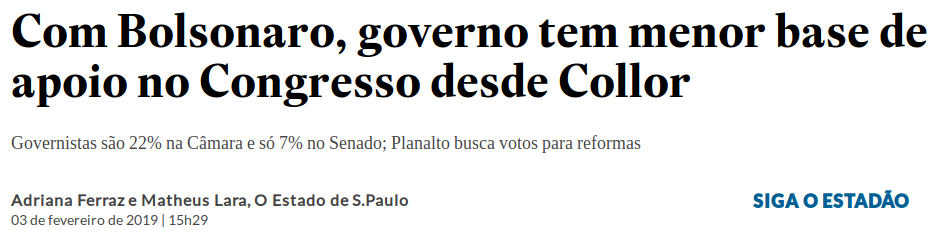
\includegraphics[width=1.0\textwidth]{manchetes/estadao-bolsonaro-menor-base.png}}
      \fbox{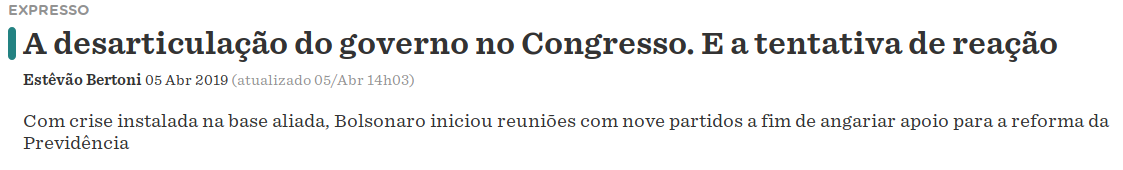
\includegraphics[width=1.0\textwidth]{manchetes/nexo-desarticulacao.png}}
      \fbox{
\includegraphics[width=1.0\textwidth]{manchetes/forum-PSL-ameaca-rebeliao.png}}
    %\end{minipage}
    %}
\caption[Exemplos de manchetes mencionando dificuldades do governo com o congresso, extraídas dos jornais
  O Estado de São Paulo e Nexo, e da Revista Fórum.]{Exemplos de manchetes mencionando dificuldades do governo com o congresso, extraídas dos jornais
  O Estado de São Paulo e Nexo, e da Revista Fórum.\footnotemark}
\label{fig:manchetes-apoio}
\end{figure}
\footnotetext{\\\myurl{http://politica.estadao.com.br/noticias/geral,com-bolsonaro-governo-tem-menor-base-de-apoio-no-congresso-desde-collor,70002706224}\\
  \myurl{http://www.nexojornal.com.br/expresso/2019/04/05/A-desarticula\%C3\%A7\%C3\%A3o-do-governo-no-Congresso.-E-a-tentativa-de-rea\%C3\%A7\%C3\%A3o}\\
  \myurl{https://www.revistaforum.com.br/parlamentares-do-psl-ameacam-rebeliao-contra-o-governo-jair-bolsonaro}}

Também analisamos o apoio ao governo por votação. A Fig. \ref{fig:apoio-governo-votacao} mostra o resultado
desse levantamento para os 100 primeiros dias das legislaturas desde 1999. Vemos que o segundo mandato
de Fernando Henrique obteve maioria absoluta em todas as votações dos 100 primeiros dias; já
o segundo mandato de Dilma é o único que não conseguiu que a média do número de votos por votação
superasse 257. Foi também nesse governo em que se registrou o maior número de votações em 100 dias.
O atual governo apresentou características típicas dos governos anteriores, com apoio médio
acima da maioria absoluta e um número mais baixo de votações.

\begin{figure}[t]
\centering
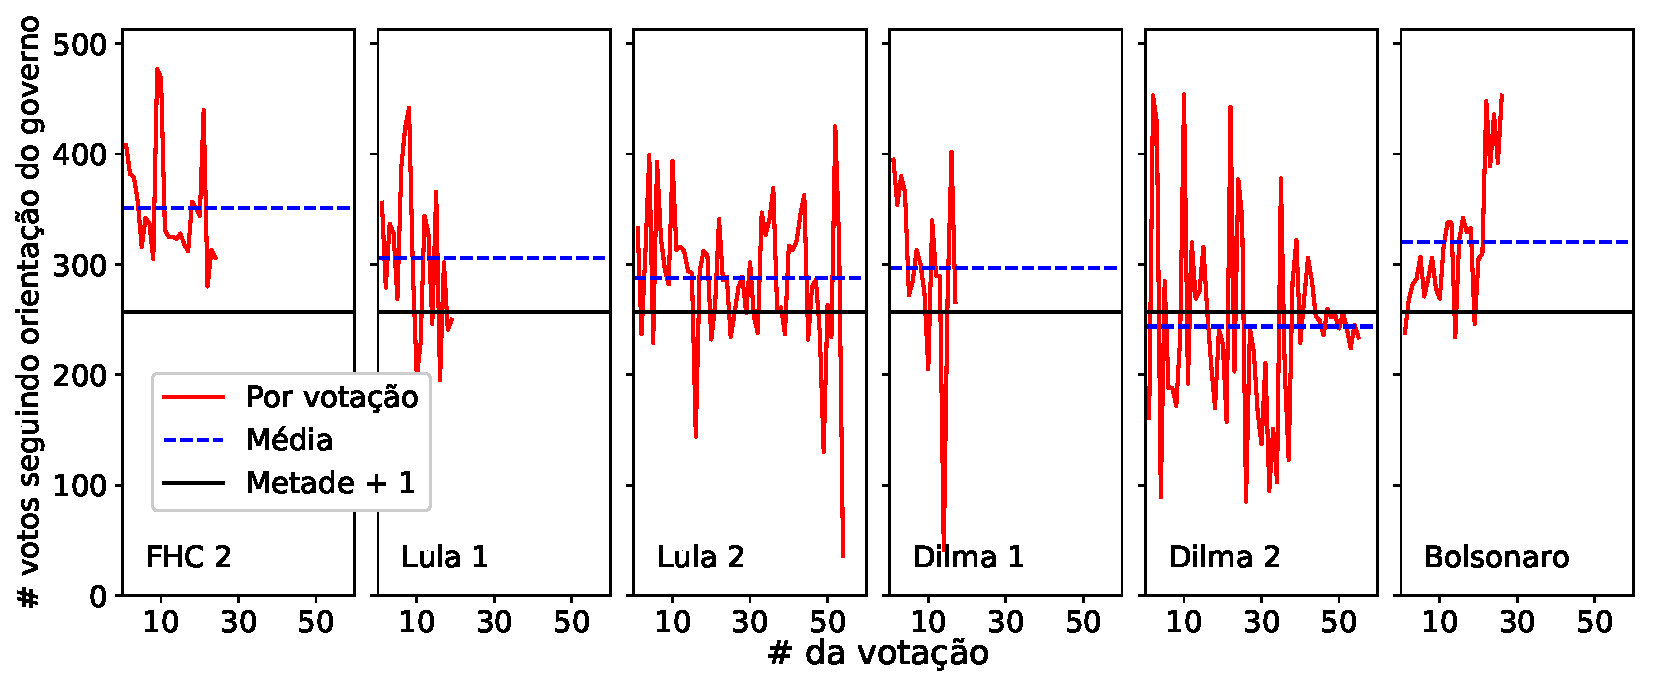
\includegraphics[width=1.0\textwidth]{graficos/apoio_ao_governo_por_votacao_2019-04-30.pdf}
\caption{Número de votos seguindo a orientação do governo, em cada votação dos 100 primeiros
  dias de congresso (em vermelho). Cada painel apresenta uma legislatura diferente, que teve
  um número diferente de votações nos 100 primeiros dias. A linha tracejada azul indica a média
  do número de votos obtidos em cada votação, e a linha contínua preta representa o mínimo de
  votos para se obter maioria absoluta (metade do total de deputados mais um).}
\label{fig:apoio-governo-votacao}
\end{figure} 

O alinhamento com o governo atual também foi estimado por partido. Nesse caso, os
partidos foram classificados de acordo com a sistematicidade com a qual seguiram
a orientação dos governos desde 1999. Aqueles que apresentaram uma taxa de apoio
superior a 2/3 em todos os governos nos quais possuíam representantes na câmara
(com exceção do segundo mandato de Dilma, que perdeu apoio de maneira generalizada) foram
denomidados ``governativos''. Partidos com presença apenas em uma legislatura, a atual (e.g. NOVO),
não foram classificados como governativos. 

A Fig. \ref{fig:apoio-governo-partido} mostra que o apoio ao governo atravessa múltiplos partidos e que,
dentre aqueles com mais de 80\% de votos, a maioria foi classificada como governativa. Nessa classificação
é importante ressalvar que alguns partidos tiveram sua composição e tamanho significativamente alterados ao longo
do tempo (e.g. PSL), de forma que seu comportamento no passado pode não ter relação com seu
comportamento atual. Do conjunto de partidos mais próximos ao governo, talvez seja mais interessante ressaltar aqueles
não classificados como governativos e que estiveram presentes em legislaturas anteriores: DEM, Cidadania (ex-PPS) e PSDB.

\begin{figure}[t]
\centering
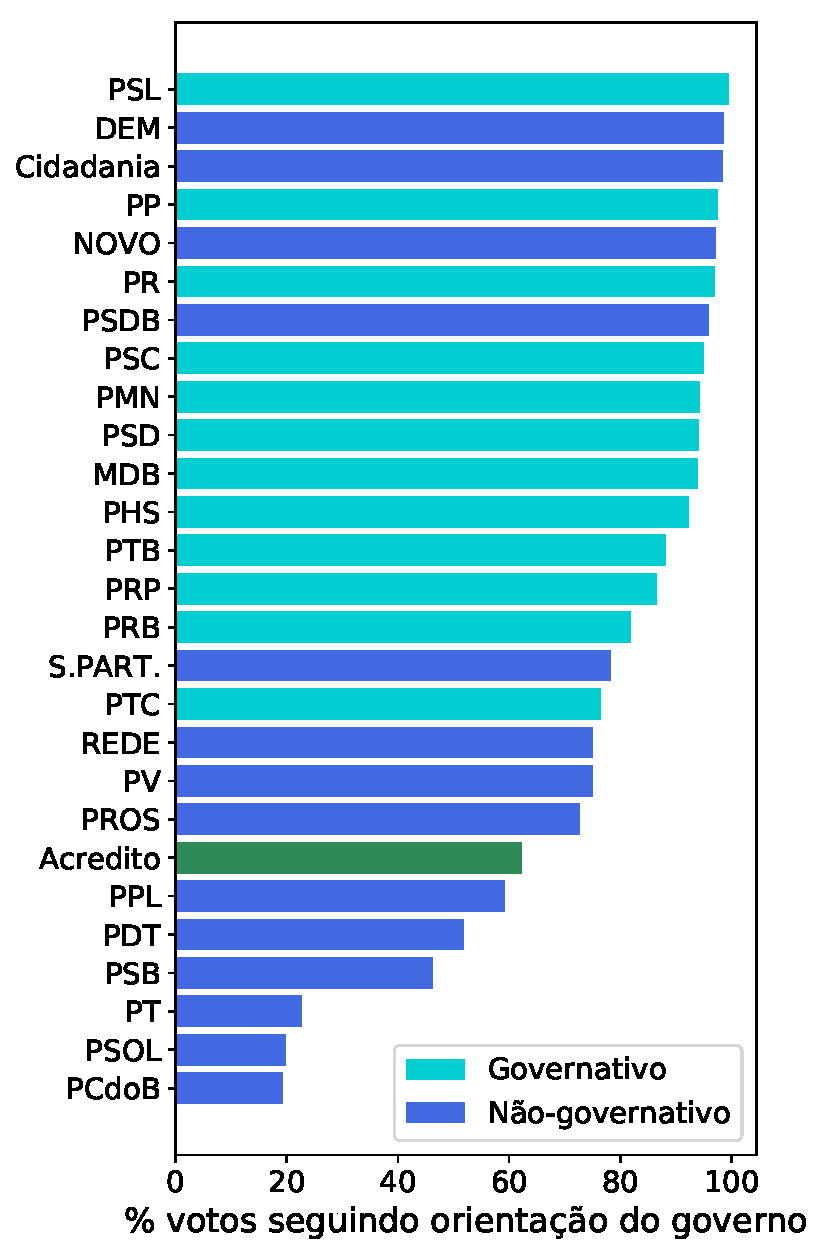
\includegraphics[width=0.55\textwidth]{graficos/apoio_ao_governo_partidos_2019-04-30.pdf}
\caption{Fração de votos dos deputados que foram alinhados com a orientação do governo atual, dentro de cada partido.
  Partidos para os quais tal fração foi superior a 2/3 no governo atual e em todos os governos nos quais tiveram representantes
  (desde 1999 e com exceção do segundo mandato de Dilma) foram denominados ``Governativos''. Partidos
  sem presença em legislatura anteriores não receberam esse rótulo.
  O conjunto de votos dos dois parlamentares do Acredito aparece em verde.}
\label{fig:apoio-governo-partido}
\end{figure} 

Vemos na Fig. \ref{fig:apoio-governo-partido} que o grau de alinhamento com o governo varia de maneira
mais ou menos suave para a maioria dos partidos. Exceção a esse comportamento se dá com o PT, PSOL e
PCdoB, que formam uma oposição mais demarcada.

\subsubsection{Fidelidade partidária}

\subsection{Distribuição de cargos e poder}
\subsection{Atividade parlamentar}


\section{Proposições}

A base de dados abertos da câmara federal indica que, nos 100 primeiros dias da atual legislatura,
foram apresentados pouco mais de 1600 projetos de lei (PLs, veja a Fig. \ref{fig:prop-2019-tipo}),
o que resulta em, aproximadamente, 3,2 projetos por deputado. Dado que os PLs são a ampla maioria
das proposições apresentadas na legislatura atual, vamos focar nossa análise nesse tipo de proposição e
compará-las com os anos anteriores.

\begin{figure}[t]
\centering
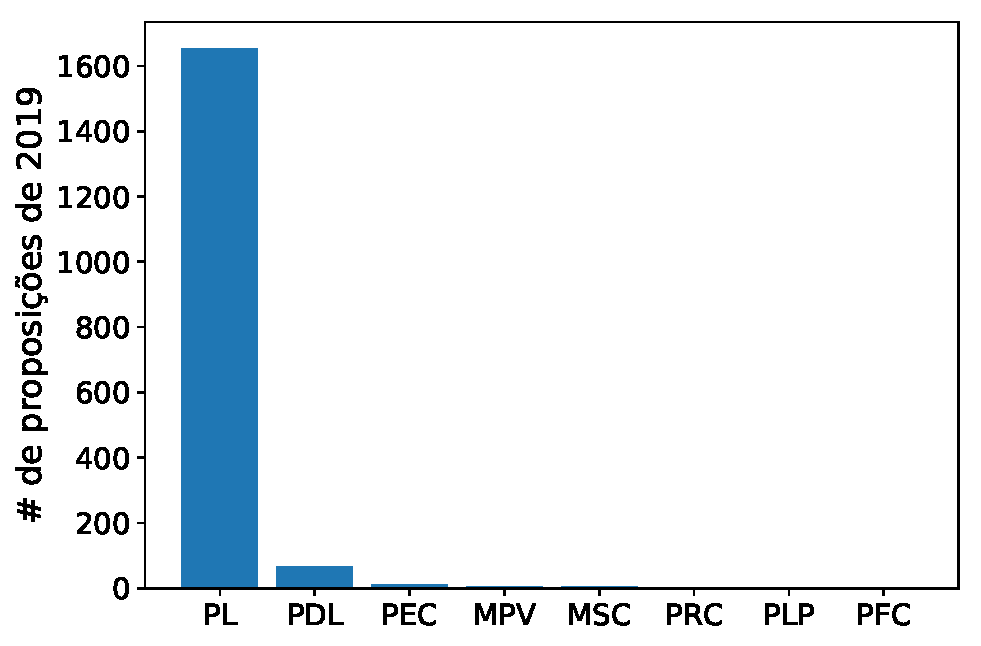
\includegraphics[width=0.7\textwidth]{graficos/proposicoes-2019-por-tipo_2019-05-01.pdf}
\caption{Número de proposições apresentadas na $56^{\mathrm{\underline{a}}}$ (atual) legislatura,
  classificadas por tipo: Projeto de Lei (PL), Projeto de Decreto Legislativo (PDL),
  Proposta de Emenda à Constituição (PEC), Medida Provisória (MPV), Mensagem de Acordos,
  convênios, tratados e atos internacionais (MSC), Projeto de Resolução da Câmara dos Deputados (PRC),
  Projeto de Lei Complementar (PLP) e Proposta de Fiscalização e Controle (PFC).}
\label{fig:prop-2019-tipo}
\end{figure} 

A Fig. \ref{fig:prop-por-ano} mostra a evolução do número de PLs apresentados ao longo do tempo,
tomando como referência o mesmo período a cada ano. Além do crescimento observado, é interessante
notar que os inícios de legislatura apresentam picos de apresentação de PLs.

\begin{figure}[t]
\centering
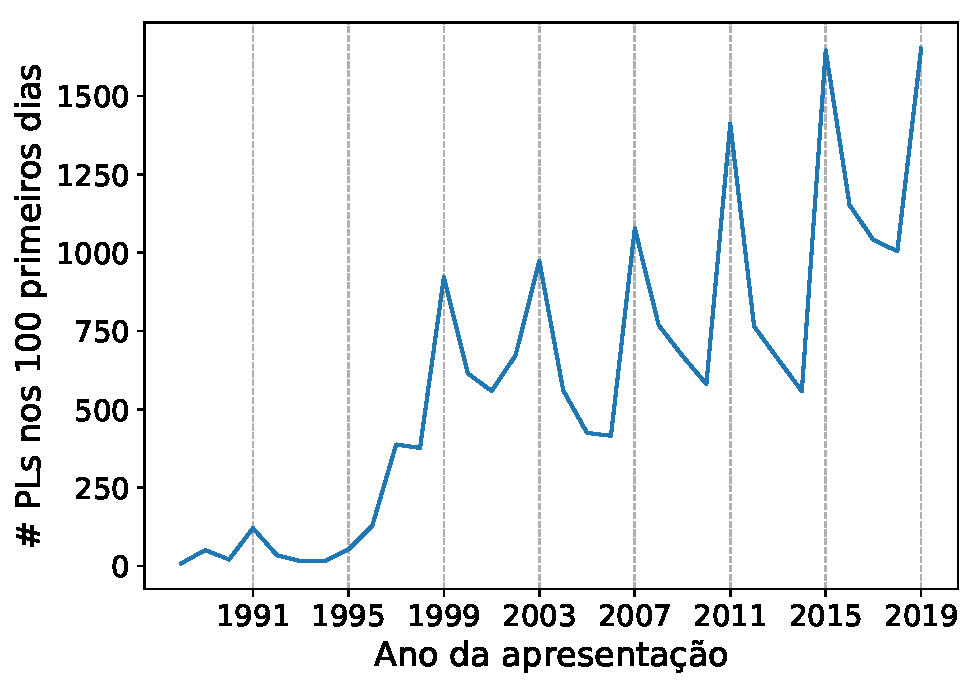
\includegraphics[width=0.7\textwidth]{graficos/PLs-por-ano_2019-05-01.pdf}
\caption{Evolução do número de PLs apresentados nos 100 dias a partir de 1 de fevereiro, de cada ano.
Os inícios de legislatura são marcados pelas linhas tracejadas cinzas.}
\label{fig:prop-por-ano}
\end{figure}

O Centro de Documentação e Informação da Câmara fornece uma classificação oficial em temas para as
proposições.\footnote{Conforme descrito em {\scriptsize\url{https://dadosabertos.camara.leg.br/swagger/api.html}}}
Nós verificamos a frequência com que cada tema apareceu em cada ano, de maneira que podemos saber
quais são os temas historicamente mais recorrentes nos projetos de lei e quais os temas mais em voga
na legislatura atual. A Fig. \ref{fig:pl-por-tema} sintetiza os resultados, na qual comparamos
a frequência de cada tema nos projetos de lei apresentados na atual legislatura com as médias das frequências
em todo o período de janeiro de 2011 a dezembro de 2018. A escolha desse período como referência
visa reduzir flutuações estatísticas (em comparação com intervalos menores de tempo) e evitar mudanças 
de comportamento abruptas e não plenamente entendidas que parecem ter ocorrido na passagem de 2010 a 2011
(conforme apresentamos abaixo).

\begin{figure}[t]
\centering
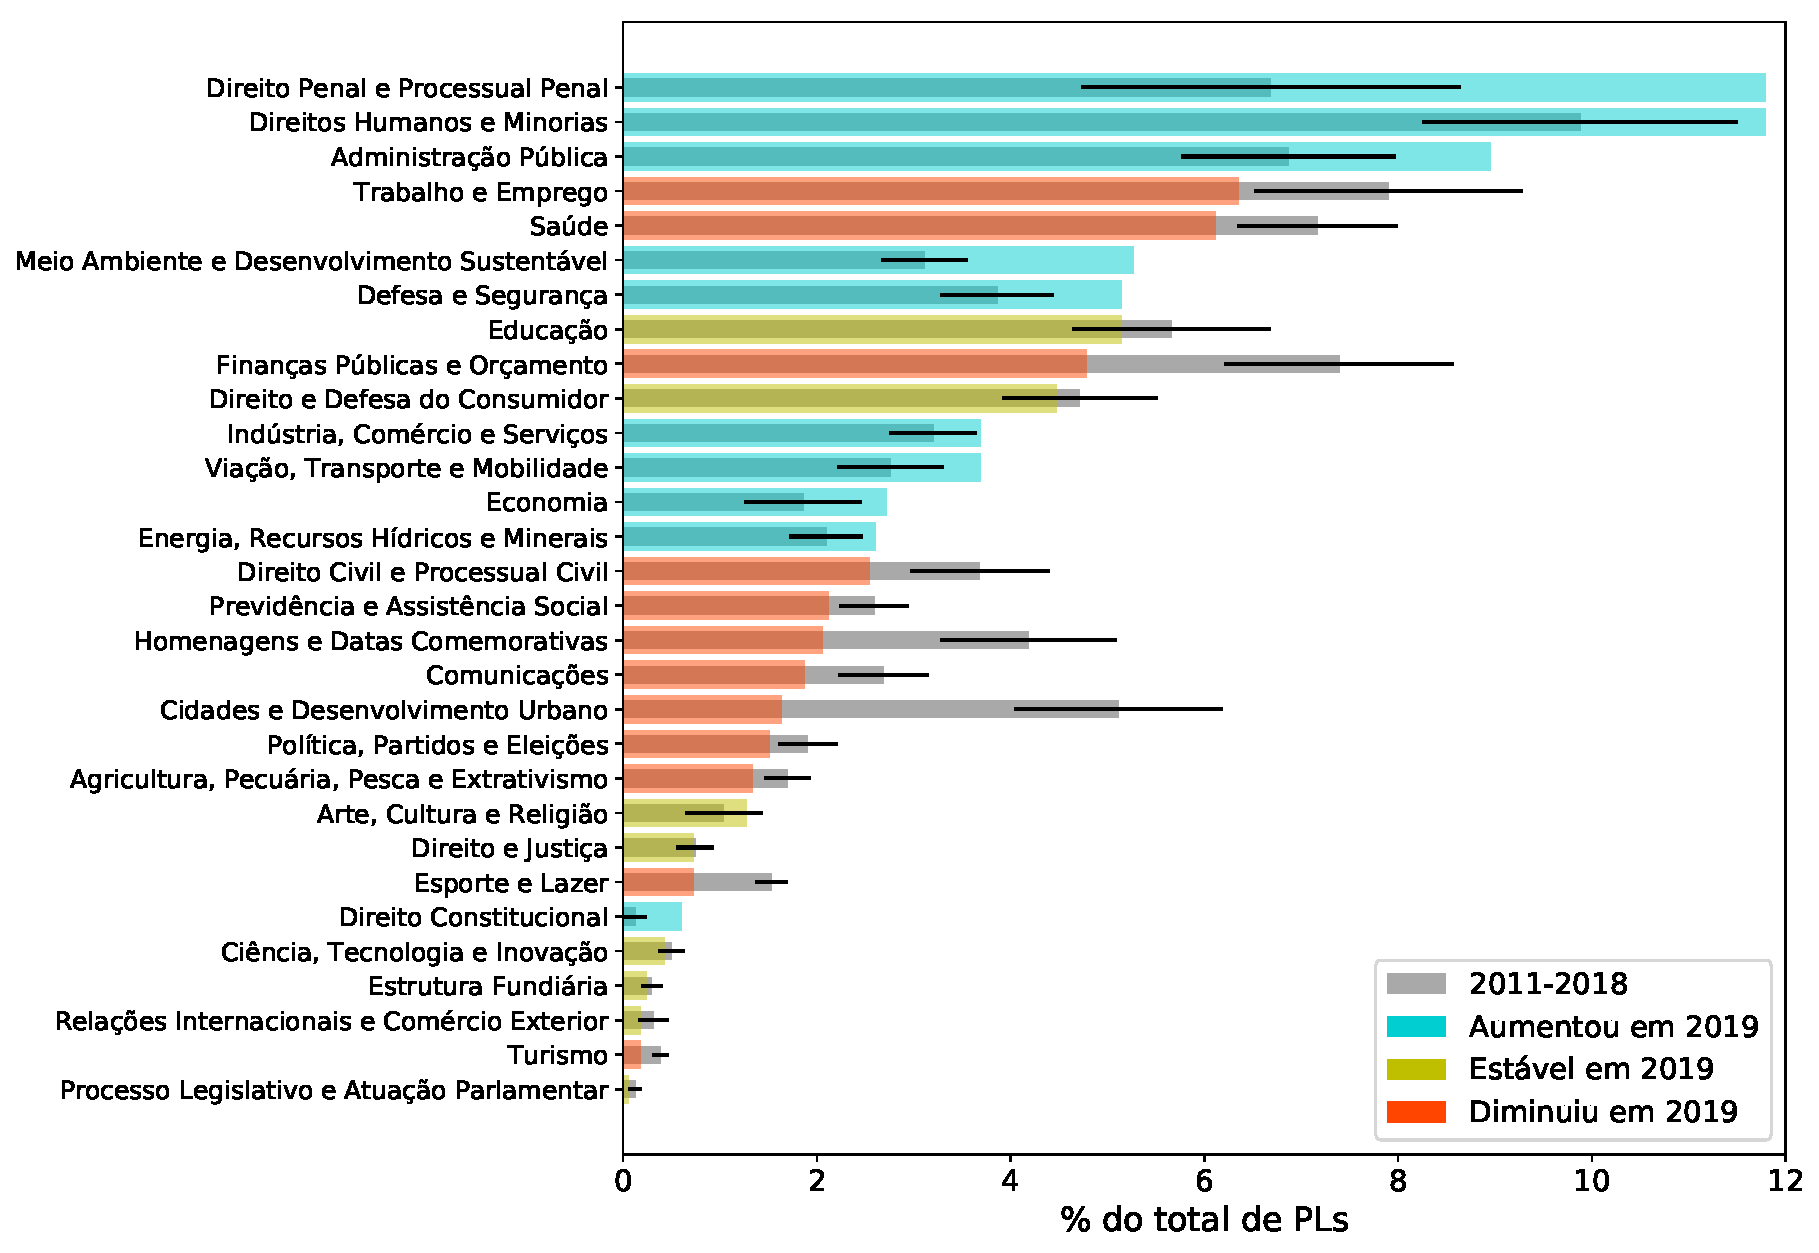
\includegraphics[width=1.0\textwidth]{graficos/temas_PL_fracao2019-vs-mediaAnterior_2019-05-01.pdf}
\caption{Frequência de cada tema (fração dos PLs apresentados que foram classificados naquele tema).
  As barras cinzas e mais estreitas representam a média da frequência no período de janeiro de 2011 a
  dezembro de 2018, e as linhas pretas indicam a variação típica (desvio padrão) da frequência no período.
  As barras coloridas representam a frequência de cada tema para os 100 dias da atual legislatura.
  Frequências que cresceram mais que a variação típica dos anos anteriores estão em azul, e as que
  diminuíram mais que a variação típica estão em vermelho. As demais são apresentadas em amarelo.
  Os temas foram ordenados pela frequência atual.}
\label{fig:pl-por-tema}
\end{figure}

Podemos notar que certos temas são, historicamente, mais frequentes que outros. No período desde 2011,
os três temas mais recorrentes foram de direitos humanos e minorias (10\%), trabalho e emprego (8\%)
e finanças públicas (7\%). Processo legislativo e atuação parlamentar, por outro lado, é tema de 0,1\%
dos PLs. Já na legislatura atual, os três temas mais comuns foram: direito penal e processual penal (12\%),
direitos humanos e minorias (12\%) e administração pública (9\%). Embora também fossem comuns nos anos
anteriores, esses temas sofreram alta, com destaque para a de direito penal e processual penal.

Os três temas que sofreram altas mais significativas foram: meio ambiente e desenvolvimento
sustentável (4,8$\sigma$, onde $\sigma$ é o desvio padrão da frequência de 2011 a 2018),
direito constitucional (4,2$\sigma$) e direito processual e penal (2,6$\sigma$). Os três
temas com baixas mais significativas foram: esporte e lazer (-4,9$\sigma$), cidades e desenvolvimento
urbano (-3,23$\sigma$) e turismo (-2,3$\sigma$). Hipotetizamos que as altas significativas
na fração de PLs apresentados indicam que os deputados estão buscando mudar as regras de jogo dentro
daquele tema em particular ou que aquele tema é prioridade para a membros da legislatura atual.
Baixas significativas podem indicar que as regras de jogo para aquele
tema são consideradas adequadas ou que o tema em questão não é prioridade para os deputados.

Conforme mencionado anteriormente, o ano de 2011 (que é um ano de início de legislatura)
marca uma mudança abrupta de comportamento para alguns temas. A Fig. \ref{fig:pl-agricultura}
exemplifica esse cenário: o tema ``estrutura fundiária'' passa de uma frequência de 2\% para outra
próxima de zero; já o tema ``Agricultura, Pecuária, Pesca e Extrativismo'' faz o caminho contrário.
Outros temas realizam transições semelhantes: direito e defesa do consumidor, direito e justiça, e
política, partidos e eleições também pulam de patamar em 2011; enquanto que viação, transporte e
mobilidade cai. Esses saltos podem indicar uma mudança na metodologia de classificação dos PLs.

\begin{figure}[t]
\centering
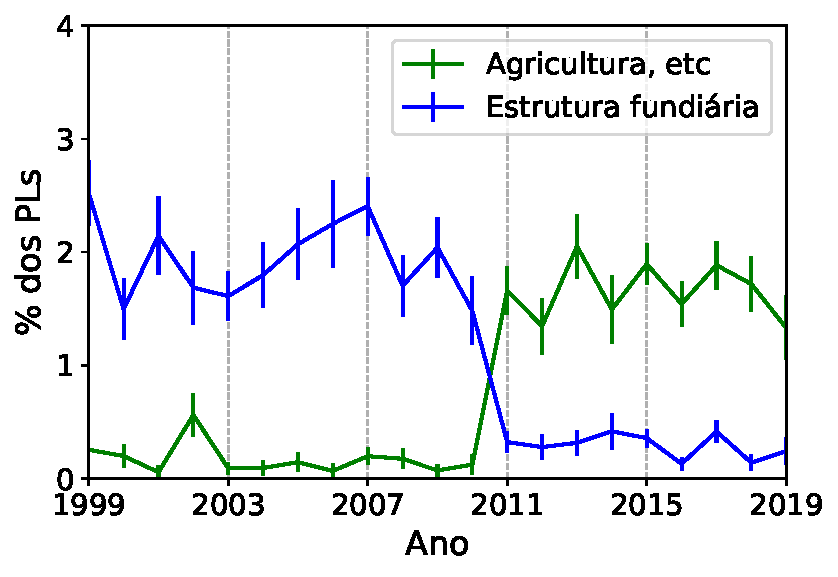
\includegraphics[width=0.6\textwidth]{graficos/PL-agricultura-por-ano_2019-05-01.pdf}
\caption{Evolução da frequência de PLs que tratam dos temas ``Agricultura, Pecuária, Pesca e Extrativismo''
  (em verde) e ``Estrutura fundiária'' (em azul), de 1999 a 2019. As barras de erro foram estimadas
assumindo que as contagems de PLs (dentro de um dado tema e de maneira agregada) sofrem flutuações de Poisson.}
\label{fig:pl-agricultura}
\end{figure}

Por fim, um achado interessante é a evolução da frequência do tema ``direitos humanos e minorias'' que,
no período analisado (de 1999 a 2019), passou por um crescimento significativo e substancial.
A Fig. \ref{fig:pl-direitos-humanos} mostra que, em 20 anos, esse tema dobrou de frequência, passando de
5\% para cerca de 11\%.

\begin{figure}[t]
\centering
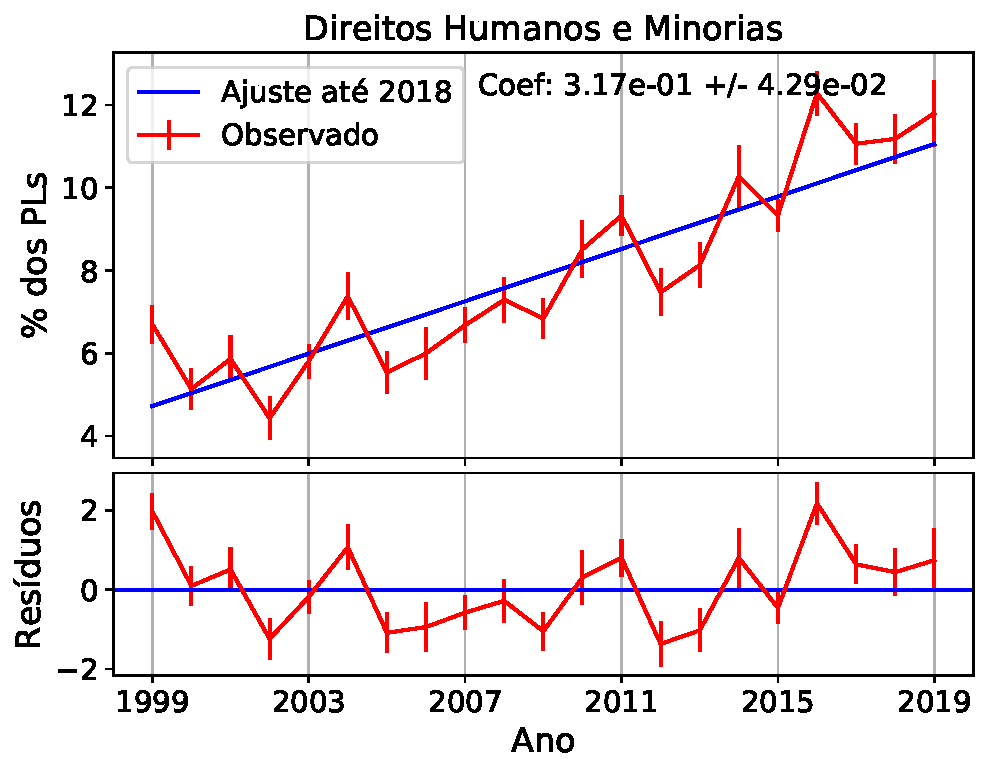
\includegraphics[width=0.7\textwidth]{graficos/PL-direitos-humanos-por-ano_2019-05-01.pdf}
\caption{O painel superior apresenta a evolução da frequência do tema ``direitos humanos e minorias''
  dentre os PLs apresentados; a linha vermelha mostra os valores observados, enquanto que a linha
  azul indica um ajuste linear com coeficiente angular $0,317\pm 0,043$. O painel inferior apresenta
  a diferença entre os valores observados e ajustados. As barras de erro foram estimadas assumindo
  flutuações de Poisson nas contagens de PLs.}
\label{fig:pl-direitos-humanos}
\end{figure}


\end{document}
